% --------------------------------------------------------------
% This is all preamble stuff that you don't have to worry about.
% Head down to where it says "Start here"
% --------------------------------------------------------------
 
\documentclass[12pt]{article}

\usepackage[latin1,utf8]{inputenc}
\usepackage[brazil]{babel}

\usepackage[margin=1in]{geometry} 
\usepackage{amsmath,amsthm,amssymb}
\usepackage{clrscode3e} % for the pseudocode
\usepackage{graphicx}
\usepackage{float}
% for the graphs %
\usepackage{tikz}
\usetikzlibrary{trees}
\usetikzlibrary{shapes,snakes}
\usepackage{verbatim}

\graphicspath{ {imgs/} }

\newcommand{\N}{\mathbb{N}}
\newcommand{\Z}{\mathbb{Z}}
 
\newenvironment{theorem}[2][Theorem]{\begin{trivlist}
\item[\hskip \labelsep {\bfseries #1}\hskip \labelsep {\bfseries #2.}]}{\end{trivlist}}
\newenvironment{lemma}[2][Lemma]{\begin{trivlist}
\item[\hskip \labelsep {\bfseries #1}\hskip \labelsep {\bfseries #2.}]}{\end{trivlist}}
\newenvironment{exercise}[2][Exercise]{\begin{trivlist}
\item[\hskip \labelsep {\bfseries #1}\hskip \labelsep {\bfseries #2.}]}{\end{trivlist}}
\newenvironment{reflection}[2][Reflection]{\begin{trivlist}
\item[\hskip \labelsep {\bfseries #1}\hskip \labelsep {\bfseries #2.}]}{\end{trivlist}}
\newenvironment{proposition}[2][Proposition]{\begin{trivlist}
\item[\hskip \labelsep {\bfseries #1}\hskip \labelsep {\bfseries #2.}]}{\end{trivlist}}
\newenvironment{corollary}[2][Corollary]{\begin{trivlist}
\item[\hskip \labelsep {\bfseries #1}\hskip \labelsep {\bfseries #2.}]}{\end{trivlist}}

\newcommand\floor[1]{\big\lfloor#1\big\rfloor}
\newcommand\ceil[1]{\big\lceil#1\big\rceil}
\newcommand\bgfrac[2]{\bigg(\dfrac{#1}{#2}\bigg)}


\begin{document}
 
% --------------------------------------------------------------
%                         Start here
% --------------------------------------------------------------
 
%\renewcommand{\qedsymbol}{\filledbox}
 
\title{MAC 5711 - Análise de Algoritmos}
\author{Rodrigo Augusto Dias Faria\\
Departamento de Ciência da Computação - IME/USP}
 
\maketitle
 
\begin{center} 
\textbf{\large{Lista 1}}
\end{center}
\noindent 1. Lembre-se que lg $n$ denota o logaritmo na base 2 de $n$. Usando a definição de notação $O$, prove que\\[6pt]
(a) $3n$ não é $O(2^n)$\\
(b) $\log_{10}n$ é $O$(lg $n$)\\
(c) lg $n$ é $O(\log_{10}n)$\\
\\[12pt]
\noindent 2. Usando a definição de notação $O$, prove que \\[6pt]
(a) $n^2 + 10n + 20 = O(n^2)$ 
\\[6pt]
Se existem as constantes $c > 0$ e $n_0 > 0$, tal que: 
\[ n^2 + 10n + 20 \leq cn^2, \forall n \geq n_0 \]
Então $n^2 + 10n + 20 = O(n^2)$. Note também a seguinte relação:
\[ n^2 + 10n + 20 \leq n^2 + 10n^2 + 20n^2 = 31n^2 \]
Logo se fizermos $c = 31$ e $n_0 = 1$ teremos que:
\[ n^2 + 10n + 20 \leq 31n^2, \forall n \geq 1 \]
Portanto podemos concluir que $n^2 + 10n + 20 = O(n^2)$. $\square$
\\[6pt]
(b) $\lceil n/3 \rceil = O(n)$
\\[6pt]
Se existem as constantes $c > 0$ e $n_0 > 0$ tal que:
\[ \lceil n/3 \rceil \leq cn, \forall n \geq n_0 \]
Então $\lceil n/3 \rceil = O(n)$. Note também a seguinte relação.
\[ \lceil \frac{n}{3} \rceil \leq \frac{n}{3} + 1 \leq \frac{n}{3} + n = \frac{4n}{3}, \forall n \geq 1 \]
Logo se fizermos $c = 4/3$ e $n_0 = 1$, teremos:
\[ \lceil n/3 \rceil \leq \frac{4n}{3}, \forall n \geq 1 \]
Portanto podemos concluir que $\lceil n/3 \rceil = O(n)$. $\square$
\\[6pt]
(c) $\lg n = O(\log_{10} n)$ 
\\[6pt]
Se existem as constantes $c > 0$ e $n_0 > 0$ tal que:
\[ \lg n \leq c \log_{10} n, \forall n \geq n_0 \]
Então $\lg n = O(\log_{10} n)$. Note que pela propriedade dos logaritmos mostrada no exercício 1-(b) podemos concluir que:
\[ \lg n = \frac{\log_{10} n}{\log_{10} 2}\]
Logo se fizermos $c = \frac{1}{\log_{10} 2}$ e $n_0 = 1$ então teremos:
\[ \lg n \leq \frac{\log_{10} n}{\log_{10} 2}, \forall n \geq 1 \]
Portanto podemos concluir que $\lg n = O(\log_{10} n)$. $\square$
\\[6pt]
(d) $n = O(2^n)$
\\[6pt]
Se existem as constantes $c > 0$ e $n_0 > 0$ tal que:
\[ n \leq 2^n, \forall n \geq n_0 \]
Então $n = O(2^n)$. Note trivialmente que se fizermos $c = 1$ e $n_0 = 1$, teremos:
\[ n \leq 2^n, \forall n \geq 1 \]
Portanto podemos concluir que $n = O(2^n)$. $\square$
\\[6pt]
(e) $n/1000$ não é $O(1)$
\\[6pt]
Vamos assumir por contradição que $n/1000 = O(1)$, e portanto que existem as constantes $c > 0$ e $n_0 > 0$ tal que:
\[ n/1000 \leq c, \forall n \geq n_0 \]
Note que quando $n \rightarrow \infty$, então $n/1000 \rightarrow \infty$, portanto não importa quão grande seja $c$, com certeza existe um $n$ suficientemente grande tal que:
\[ n/1000 > c\]
Logo podemos concluir que $n/1000 \not \in O(1)$. $\square$.
\\[6pt]
(f) $n^2/2$ não é $O(n)$
\\[6pt]
Vamos assumir por contradição que $n^2/2 = O(n)$, e portanto que existem as constantes $c > 0$ e $n_0 > 0$ tal que:
\[ n^2/2 \leq  cn, \forall n \geq n_0 \]
Dividindo os dois lados por $n$ teremos:
\begin{align*}
  \frac{n^2}{2n} &\leq \frac{cn}{n}, \forall n \geq n_0 \\
  \frac{n}{2} &\leq c, \forall n \geq n_0
\end{align*}
Note que quando $n \rightarrow \infty$, então $\frac{n}{2} \rightarrow \infty$, portanto não importa quão grande seja $c$ com certeza existe um $n$ suficientemente grande tal que:
\[ n^2/2 > cn \]
Portanto podemos concluir que $n^2/2$ não é $O(n)$. $\square$







\clearpage
\begin{center} 
\textbf{\large{Lista 2}}
\end{center}
\\[12pt]
\noindent 2. Usando a definição de notação $O$, prove que \\[6pt]
(a) $n^2 + 10n + 20 = O(n^2)$ 
\\[6pt]
Se existem as constantes $c > 0$ e $n_0 > 0$, tal que: 
\[ n^2 + 10n + 20 \leq cn^2, \forall n \geq n_0 \]
Então $n^2 + 10n + 20 = O(n^2)$. Note também a seguinte relação:
\[ n^2 + 10n + 20 \leq n^2 + 10n^2 + 20n^2 = 31n^2 \]
Logo se fizermos $c = 31$ e $n_0 = 1$ teremos que:
\[ n^2 + 10n + 20 \leq 31n^2, \forall n \geq 1 \]
Portanto podemos concluir que $n^2 + 10n + 20 = O(n^2)$. $\square$
\\[6pt]
(b) $\lceil n/3 \rceil = O(n)$
\\[6pt]
Se existem as constantes $c > 0$ e $n_0 > 0$ tal que:
\[ \lceil n/3 \rceil \leq cn, \forall n \geq n_0 \]
Então $\lceil n/3 \rceil = O(n)$. Note também a seguinte relação.
\[ \lceil \frac{n}{3} \rceil \leq \frac{n}{3} + 1 \leq \frac{n}{3} + n = \frac{4n}{3}, \forall n \geq 1 \]
Logo se fizermos $c = 4/3$ e $n_0 = 1$, teremos:
\[ \lceil n/3 \rceil \leq \frac{4n}{3}, \forall n \geq 1 \]
Portanto podemos concluir que $\lceil n/3 \rceil = O(n)$. $\square$
\\[6pt]
(c) $\lg n = O(\log_{10} n)$ 
\\[6pt]
Se existem as constantes $c > 0$ e $n_0 > 0$ tal que:
\[ \lg n \leq c \log_{10} n, \forall n \geq n_0 \]
Então $\lg n = O(\log_{10} n)$. Note que pela propriedade dos logaritmos mostrada no exercício 1-(b) podemos concluir que:
\[ \lg n = \frac{\log_{10} n}{\log_{10} 2}\]
Logo se fizermos $c = \frac{1}{\log_{10} 2}$ e $n_0 = 1$ então teremos:
\[ \lg n \leq \frac{\log_{10} n}{\log_{10} 2}, \forall n \geq 1 \]
Portanto podemos concluir que $\lg n = O(\log_{10} n)$. $\square$
\\[6pt]
(d) $n = O(2^n)$
\\[6pt]
Se existem as constantes $c > 0$ e $n_0 > 0$ tal que:
\[ n \leq 2^n, \forall n \geq n_0 \]
Então $n = O(2^n)$. Note trivialmente que se fizermos $c = 1$ e $n_0 = 1$, teremos:
\[ n \leq 2^n, \forall n \geq 1 \]
Portanto podemos concluir que $n = O(2^n)$. $\square$
\\[6pt]
(e) $n/1000$ não é $O(1)$
\\[6pt]
Vamos assumir por contradição que $n/1000 = O(1)$, e portanto que existem as constantes $c > 0$ e $n_0 > 0$ tal que:
\[ n/1000 \leq c, \forall n \geq n_0 \]
Note que quando $n \rightarrow \infty$, então $n/1000 \rightarrow \infty$, portanto não importa quão grande seja $c$, com certeza existe um $n$ suficientemente grande tal que:
\[ n/1000 > c\]
Logo podemos concluir que $n/1000 \not \in O(1)$. $\square$.
\\[6pt]
(f) $n^2/2$ não é $O(n)$
\\[6pt]
Vamos assumir por contradição que $n^2/2 = O(n)$, e portanto que existem as constantes $c > 0$ e $n_0 > 0$ tal que:
\[ n^2/2 \leq  cn, \forall n \geq n_0 \]
Dividindo os dois lados por $n$ teremos:
\begin{align*}
  \frac{n^2}{2n} &\leq \frac{cn}{n}, \forall n \geq n_0 \\
  \frac{n}{2} &\leq c, \forall n \geq n_0
\end{align*}
Note que quando $n \rightarrow \infty$, então $\frac{n}{2} \rightarrow \infty$, portanto não importa quão grande seja $c$ com certeza existe um $n$ suficientemente grande tal que:
\[ n^2/2 > cn \]
Portanto podemos concluir que $n^2/2$ não é $O(n)$. $\square$





\noindent 2. Escreva um algoritmo que ordena uma lista de n itens dividindo-a em três sublistas de aproximadamente $n/3$ itens, ordenando cada sublista recursivamente e intercalando as três sublistas ordenadas. Analise seu algoritmo concluindo qual é o seu consumo de tempo.\\[6pt]
Para este exercício, devemos efetuar uma alteração no $\proc{Mergesort}$ para a divisão do vetor $A$ em três partições utilizando o $\proc{Merge}$ duas vezes ao final para intercalar as três partes ordenadas em um único vetor.

\begin{codebox}
\Procname{$\proc{Mergesort3}(A, p, r)$}
\li    \If $p < r$
\li         \Then
            $k = \floor{(p + r) / 3}$
\li         $m = k+1 + \floor{(p + r) / 3}$
\li         $\proc{Mergesort3}(A, p, k)$
\li         $\proc{Mergesort3}(A, k + 1, m)$
\li         $\proc{Mergesort3}(A, m + 1, r)$
\li         $\proc{Merge}(A, p, k, m)$
\li         $\proc{Merge}(A, p, m, r)$
            \End
\End
\end{codebox}

\textbf{Consumo de tempo}\\[6pt]
As linhas 1-3 consomem $\Theta(1)$. As linhas 4-5 têm consumo $T(\ceil{n / 3})$ e a linha 6 tem consumo $T(n - \ceil{2n / 3})$, já que a terceira partição não tem tamanho exatamente de $\ceil{n / 3}$. Sabemos que o consumo do $\proc{Merge}$ é $\Theta(n)$, logo:\\
\begin{align*}
T(n) & = T(\ceil{n / 3}) + T(\ceil{n / 3}) + T(n - 2\ceil{n / 3}) + \Theta(n) + \Theta(n) \\
& = 2T(\ceil{n / 3}) + T(\ceil{n / 3}) + \Theta(2n) \\
& = 3T(\ceil{n / 3}) + \Theta(2n)
\end{align*}

Como $\Theta(2n)$ é $\Theta(n)$:\\
\begin{align*}
T(n) & = 3T(\ceil{n / 3}) + \Theta(n)
\end{align*}

Simplificando a recorrência, temos:\\
\begin{eqnarray*}
T(n) = \left\{ \begin{array}{rl} 
 1, &\mbox{ $n = 1$} \\
 3T\bgfrac{n}{3} + n, &\mbox{ $n >= 2 $ potência de 2}
       \end{array} \right.
\end{eqnarray*}

Por expansão:\\
\begin{align*}
T(n) & = 3T\bgfrac{n}{3} + n\\
&= 3 \bigg( 3T\bgfrac{n}{3^2} + \bgfrac{n}{3} \bigg) + n &= 3^2T\bgfrac{n}{3^2} + n + n\\
&= 3^2 \bigg( 3T\bgfrac{n}{3^3} + \bgfrac{n}{3^2} \bigg) + n + n &= 3^3T\bgfrac{n}{3^3} + n + n + n\\
&= ... \\
&= 3^kT\bgfrac{n}{3^k} + kn
\end{align*}

Assumindo $k = \log_3{n}$ e $3^k = n$:\\
\begin{align*}
T(n) &= nT\bgfrac{n}{n} + \log_3{n}\\
&= T(1)n + \log_3{n}(n)\\
&= n + n(\log_3{n})\\
\end{align*}

Portanto, $T(n) = n + n(\log_3{n})$ é $\Theta(n\log{n})$.

\begin{proof}
Prova por indução em k.

\textbf{Base:} para $n = 1$
\begin{align*}
T(1) = 1 = 1 + 1(\log_3{1}) = 1+ 0 = 1
\end{align*}

\textbf{Hipótese de Indução:} Assuma que $T(x) = x + x(\log_3{x})$ vale para $1 >= x < n$\\

\textbf{Passo:} para $n >= 2$
\begin{align*}
T(n) = 3T\bgfrac{n}{3} + n &= 3\bigg( \bgfrac{n}{3} + \bgfrac{n(\log_3{\frac{n}{3}})}{3} \bigg) + n & (\text{por HI})\\
&= 3\bgfrac{n}{3} + 3\bigg( \bgfrac{n}{3}\log_3{\frac{n}{3}}\bigg) + n\\
&= n + n + n\log_3{\frac{n}{3}}\\
&= 2n + n\log_3{n} - n\\
&= n + n\log_3{n}
\end{align*}

Como queríamos demonstrar!

\end{proof}

\clearpage
\begin{center} 
\textbf{\large{Lista 3}}
\end{center}

\noindent 2. Qual é o consumo de espaço do QUICKSORT no pior caso?\\[6pt]
A avaliação de um algoritmo quanto ao consumo de espaço está relacionada com a necessidade de alocação de espaço adicional na pilha de recursão.

No pior caso, o QUICKSORT será executado uma vez para cada elemento da lista dada de tamanho $n$, ou seja, teremos $n$ chamadas recursivas.

Isso significa que, com uma lista de $n$ elementos, $n$ novas chamadas serão adicionadas à pilha no pior caso, o que nos leva a uma complexidade de espaço O($n$).

\noindent 3. Quando um algoritmo recursivo tem como último comando executado, em algum de seus casos, uma chamada recursiva, tal chamada é denominada recursão de calda (\textit{tail recursion}). Um exemplo de recursão de calda acontece no QUICKSORT.
\begin{codebox}
\Procname{$\proc{Quicksort}(A, p, r)$}
\li     q = \proc{Partition}(A, p, r)
\li     \proc{Quicksort}(A, p, q - 1)
\li     \proc{Quicksort}(A, q + 1, r)
\End
\end{codebox}

Toda recursão de calda pode ser substituída por uma repetição. No caso do $\proc{Quicksort}$, obtemos o seguinte:
\begin{codebox}
\Procname{$\proc{Quicksort}(A, p, r)$}
\li     \While $p < r$
\li         \Do
                $q \gets \proc{Partition}(A, p, r)$
\li             \proc{Quicksort}(A, p, q - 1)
\li             $p \gets q + 1$
            \End
\end{codebox}

Mostre como essa ideia pode ser usada (de uma maneira mais esperta) para melhorar significativamente o consumo de espaço no pior caso do $\proc{Quicksort}$.\\[6pt]
O benefício da utilização do loop ao invés da recursão de cauda é que, geralmente, precisamos de menos memória na pilha para ordenar todos os elementos do vetor $A$, já que a implementação sem a recursão de cauda reusa o ambiente da pilha (variáveis locais, parâmetros, etc) a cada iteração.

A profundidade das chamadas recursivas está relacionada com a ordem em que os elementos se encontram. Se, por exemplo, o vetor $A$ está em ordem decrescente, teremos a execução no pior caso. Isso implica na forma em que cada partição é gerada.

Para ter um resultado ainda mais eficiente, os intervalos podem ser comparados para se certificar de que a maior partição é sempre processada de forma iterativa e a menor de forma recursiva, o que garante a menor profundidade de recursão possível para um determinado vetor de entrada e pivô.
\begin{codebox}
\Procname{$\proc{Half-Tail-Quicksort}(A, p, r)$}
\li     \While $p < r$
\li         \Do
                $q \gets \proc{Partition}(A, p, r)$
\li             \If $(q - p) < (r - q)$
\li                 \Then
                    \proc{Half-Tail-Quicksort}(A, p, q - 1)
\li                 $p \gets q + 1$
\li                 \Else
\li                 \proc{Half-Tail-Quicksort}(A, q + 1, r)
\li                 $r \gets q - 1$
                \End
            \End
\end{codebox}


\noindent 4. Considere o seguinte algoritmo que determina o segundo maior elemento de um vetor $v[1..n]$ com $n>=2$ números positivos distintos.\\[6pt]
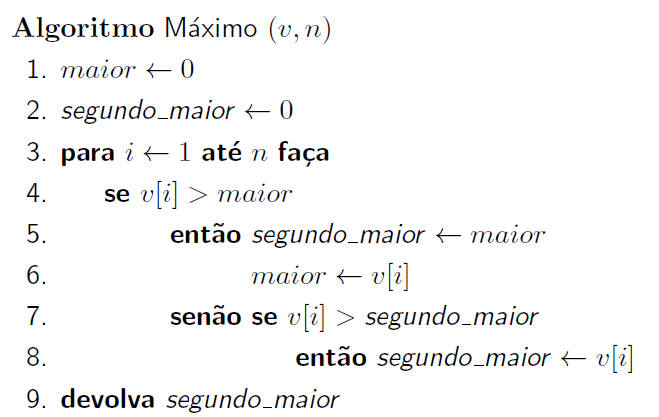
\includegraphics[width=0.6\textwidth]{algo3-4.png}

Suponha que a entrada do algoritmo é uma permutação de 1 a $n$ escolhida uniformemente dentre todas as permutaçõees de 1 a $n$.
Qual é o número esperado de comparações executadas na linha 6 do algoritmo? Qual é o número esperado de atribuições efetuadas na linha 7 do algoritmo?

Vamos calcular $E[X]$ para o algoritmo dado. Seja:\\
A = número de vezes que a linha 5 do algoritmo foi executada\\
B = número de vezes que a linha 8 do algoritmo foi executada\\

X = A + B

\begin{eqnarray*}
X_i = \left\{ \begin{array}{rl} 
 1, &\mbox{ se A ou B} \\
 0, &\mbox{ c.c}
       \end{array} \right.
\end{eqnarray*}

Logo:\\
$E[X_i] = 0 * Pr\{X_i = 0\} + 1 * Pr\{X_i = 1\} = Pr\{X_i = 1\}$\\

Sabemos que a execução da linha 8 depende da avaliação da linha 5, logo:\\
$E[X_i] = Pr\{A\} + (1 - Pr\{A\})*Pr\{B|\bar{A}\}$\\

Como já vimos para a versão original do algoritmo $\proc{Máximo}$ é $Pr\{A\} = \dfrac{1}{i}$.\\
Para a probabilidade de execução da linha 8, temos que:\\
$Pr\{B|\bar{A}\} = \dfrac{1}{1 - i}$\\

Portanto:
\begin{align*}
E[X_i] &= \bgfrac{1}{i} + \bigg(1 - \dfrac{1}{i}\bigg)\bigg(\dfrac{1}{i - 1}\bigg) \\
&= \bgfrac{1}{i} + \bigg(\dfrac{i - 1}{i}\bigg)\bigg(\dfrac{1}{i - 1}\bigg) \\
&= \dfrac{2}{i}
\end{align*}

É fato que a linha 5 sempre será executada na primeira iteração, assumindo que $v[1..n]$ contenha apenas inteiros positivos e $n >= 2$. Logo:
\begin{align*}
E[X_i] &= 1 + \sum_{i=2}^{n} \dfrac{2}{i} = 1 + 2\sum_{i=2}^{n} \dfrac{1}{i}
\end{align*}

\noindent 6. (\textbf{CLRS 8.4-3}) Seja X uma variável aleatória que é igual ao número de caras em duas jogadas de uma moeda justa. Quanto vale $E[X^2]$? Quanto vale $E[X]^2$?\\[6pt]

\begin{eqnarray*}
X = \left\{ \begin{array}{rl} 
 1, &\mbox{ se temos cara} \\
 0, &\mbox{ c.c}
       \end{array} \right.
\end{eqnarray*}

A probabilidade de cada evento elementar é:\\
$Pr\{X = cara\} = \dfrac{1}{2}$\\
$Pr\{X = coroa\} = \dfrac{1}{2}$\\

Vamos agora calcular $E[X^2]$:
\begin{eqnarray*}
  E[X^2] &=& 0^2 * \frac{1}{2} + 1^2 * \frac{1}{2}  \\
  &=& \frac{1}{2}
\end{eqnarray*}

e para $E^2[X]$, temos:
\begin{eqnarray*}
E^2[X] &=& E[X]*E[X] \\
&=& \dfrac{1}{2} * \dfrac{1}{2}\\
&=& \dfrac{1}{4}
\end{eqnarray*}
\clearpage

\begin{center} 
\textbf{\large{Lista 4}}
\end{center}

\noindent 1. Escreva uma função que recebe um vetor com n letras A’s e B’s e, por meio de trocas, move todos os A’s para o início do vetor. Sua função deve consumir tempo O($n$).\\[6pt]
Resposta\\
\input{q4-2}

\noindent 3. Sejam $X[1..n]$ e $Y[1..n]$ dois vetores, cada um contendo $n$ números ordenados. Escreva um algoritmo O(lg $n$) para encontrar uma das medianas de todos os $2n$ elementos nos vetores $X$ e $Y$.\\[6pt]
Sabemos que a mediana de X e Y está em $i = \floor{q / 2}$ e $j = \floor{s / 2}$, respectivamente. Note que $n = q + s$ é par, e é por isso que nós estamos usando a função \textbf{piso}.

Se $X[i]$ é maior do que $Y[j]$, significa que a mediana global está à esquerda de $X[i]$ e à direita de $Y[j]$. Se $X[i]$ é menor ou igual a $Y[j]$, nós procuramos a mediana à esquerda de $Y[j]$ e à direita de $X[i]$.

A condição de parada dá-se quando $p == q$, o que significa que a mediana global está dentro do vetor $X$. Caso contrário, se $r == s$, a mediana está em $Y$.

O pseudocódigo $\proc{Find-Median}$ mostra a operação descrita acima que, também, é o resultado do exercício 9.3-8 CLRS 3ed.\\

\begin{codebox}
\Procname{$\proc{Find-Median}(X, Y, p, q, r, s)$}
\li \If $p \isequal q$
\li \Comment We have found the median between p, q and r
\li     \Then
            \Return $X[p]$
\li     \ElseIf $r \isequal s$
\li \Comment We have found the median between q, r and s
\li     \Then
            \Return $Y[r]$
        \End
\li $i \gets p + (q - p) / 2$
\li $j = r + (s - r) / 2$
\li \If $X[i] > Y[j]$
\li     \Then
            $q \gets i$
\li         $r \gets j$
\li     \Else
\li         $p \gets i$
\li         $s \gets j$
        \End
\li \Return $\proc{Find-Median}(X, Y, p, q, r, s)$
\End
\end{codebox}
\noindent 4. (\textbf{CLRS 9.3-5}) Para esta questão, vamos dizer que a mediana de um vetor $A[p..r]$ com números inteiros é o valor que ficaria na posição $A[\floor{(p + r)/2}]$ depois que o vetor $A[p..r]$ fosse ordenado.\\
Dado um algoritmo linear “caixa-preta” que devolve a mediana de um vetor, descreva um algoritmo simples, linear, que, dado um vetor $A[p..r]$ de inteiros distintos e um inteiro $k$, devolve o \textit{k-ésimo} mínimo do vetor. (O \textit{k-ésimo} mínimo de um vetor de inteiros distintos é o elemento que estaria na \textit{k-ésima} posição do vetor se ele fosse ordenado.)\\[6pt]
Resposta\\

\noindent 8. (\textbf{CLRS 8.3-2}) Quais dos seguintes algoritmos de ordenação são estáveis: insertionsort, mergesort, heapsort, e quicksort. Descreva uma maneira simples de deixar qualquer algoritmo de ordenação estável. Quanto tempo e/ou espaço adicional a sua estratégia usa?\\[6pt]
Os algoritmos estáveis são o insertionsort e o mergesort (versão do Cormen). Os demais não são estáveis.

Uma forma simples de deixar qualquer algoritmo de ordenação estável é criar um mecanismo de indexação que mantenha a ordem em que os elementos aparecem originalmente, ou seja, basta termos um índice para cada elemento de um vetor de $n$ elementos.

Esse mecanismo necessita de $\Theta(n)$ espaço extra para armazenar os $n$ índices do vetor de $n$ elementos.\\

\clearpage

\begin{center} 
\textbf{\large{Lista 5}}
\end{center}


\noindent 1. Desenhe a árvore de decisão para o $\proc{Selectionsort}$ aplicado a $A[1..3]$ com todos os elementos distintos.\\[6pt]
% Set the overall layout of the tree
\tikzstyle{level 1}=[level distance=1.5cm, sibling distance=6cm]
\tikzstyle{level 2}=[level distance=1.5cm, sibling distance=3cm]
\tikzstyle{level 3}=[level distance=1.5cm, sibling distance=3cm]

% Define styles for bags and leafs
\tikzstyle{bag} = [shape=ellipse, draw, align=center,
                   top color=white, bottom color=gray!20]
\tikzstyle{end} = [shape=rectangle, rounded corners, draw, align=center, fill=gray!40]

\begin{tikzpicture}[grow=down]
\node[bag] {1:2}
    child {
        node[bag] {2:3}        
            child {
                node[end]{$\langle 3, 2, 1 \rangle$}
                edge from parent
                node[above] {$\geq$}
            }
            child {
                node[bag] {1:3}
                	child {
                        node[end]{$\langle 3, 1, 2 \rangle$}
                        edge from parent
                        node[above] {$\geq$}
                    }
                	child {
                        node[end]{$\langle 2, 1, 3 \rangle$}
                        edge from parent
                        node[above] {$<$}
                    }
                edge from parent 
                node[above] {$<$}
			}
            edge from parent 
            node[above] {$\geq$}
    }
    child {
        node[bag] {1:3}        
            child {
                node[end]{$\langle 2, 3, 1 \rangle$}
                edge from parent
                node[above] {$\geq$}
            }
            child {
                node[bag] {2:3}
                	child {
                        node[end]{$\langle 1, 3, 2 \rangle$}
                        edge from parent
                        node[above] {$\geq$}
                    }
                	child {
                        node[end]{$\langle 1, 2, 3 \rangle$}
                        edge from parent
                        node[above] {$<$}
                    }
                edge from parent 
                node[above] {$<$}
			}
            edge from parent 
            node[above] {$<$}
    };
\end{tikzpicture}\\

\noindent 2. \textbf{(CLRS 8.1-1)} Qual a menor profundidade (= menor nível) que uma folha pode ter em uma árvore de decisão que descreve um algoritmo de ordenação baseado em comparações?\\[6pt]
A menor profundidade da árvore de decisão é, coincidentemente, a cota inferior das alturas de todas as árvores de decisão nas quais aparecem uma folha (uma das $n!$ permutações da entrada).

Também podemos dizer que é o melhor caso em tempo de execução de qualquer algoritmo de ordenação baseado em comparações.

Logo, é o caso em que apenas $n - 1$ comparações são realizadas para ordenar o vetor que ocorre, por exemplo, quando o vetor já está ordenado.\\[12pt]

\noindent 3. Mostre que $lg(n!) \geq \frac{n}{4} lg n$ para $n \geq 4$ sem usar a fórmula de Stirling.\\[6pt]
$n!$ pode ser escrito como um produtório:
\begin{align*}
\prod_{k=1}^n k
\end{align*}

Também podemos escrever o produtório como um somatório, pela seguinte identidade (CLRS pp 1061 - 2ed):
\begin{align*}
lg\big(\prod_{k=1}^n k\big) = \sum_{k=1}^n lg(k)
\end{align*}

Logo:
\begin{align*}
lg(n!) = \sum_{k=1}^n lg(k) &= \sum_{k=1}^{\floor{\frac{n}{4}}} lg(k) + \sum_{k=\floor{\frac{n}{4}} + 1}^{2\floor{\frac{n}{4}}} lg(k) + \sum_{k=2\floor{\frac{n}{4}} + 1}^{3\floor{\frac{n}{4}}} lg(k) + \sum_{k=3\floor{\frac{n}{4}} + 1}^{n} lg(k) \\
&\geq \sum_{k=\floor{\frac{n}{4}} + 1}^{n} lg(k) & \text{(descartando 1/4 da soma)} \\
&\geq \sum_{k=\frac{n}{4}}^n lg(\frac{n}{4}) \\
&\geq \frac{n}{4}lg\frac{n}{4} = \frac{n}{4}(lg n - lg 2^2) = \frac{n}{4}(lg n - 2) = \frac{n}{4}lg n - \frac{1}{2}n\\\\
\therefore lg(n!) \geq \frac{n}{4}lg n
\end{align*}



\noindent 4. (\textbf{CLRS 8.1-3}) Mostre que não há algoritmo de ordenação 
baseado em comparações cujo consumo de tempo é linear para pelo menos metade de 
$n!$ permutações de 1 a $n$. O que acontece se trocarmos "metade" por uma fração 
de $1/n$? O que acontece se trocarmos "metade" por uma fração de $1/2^n$?
\\ [6pt]
\textbf{Resposta:} Assim como visto em aula uma árvore de decisão pode ser 
utilizada para representar o número de comparações executadas por um algoritmo. 
A árvore de decisão é uma árvore binária onde cada nó não folha é uma comparação 
e cada folha é uma permutação de entrada, o caminho da raiz da árvore até uma de 
suas folhas mostra a quantidade de comparações executadas para aquela 
permutação, portanto a distância da raiz para a folha mais distânte (altura da 
árvore) reflete o tempo gasto pelo pior caso do algoritmo.
\\[6pt]
Vamos verificar qual a altura da árvore de decisão para saber qual o tempo gasto 
no pior caso para pelo menos metade das possíveis permutações $n!/2$. Seja $l$ o 
número de folhas do algoritmo e $h$ a altura da árvore, como a árvore de decisão 
é uma árvore binária sabemos que ela terá no máximo $2^h$ folhas. Portanto temos 
a seguinte relação:
\[ \frac{n!}{2} \leq l \leq 2^h \]
Calculando o logaritmo dos dois lados e sabendo que logaritmo é uma função 
monotonicamente crescente temos que:
\begin{align*}
     \lg 2^h  &\geq  \lg \frac{n!}{2} \\
     h & \geq \lg n! - \lg 2 \\
     h & \geq \lg n! - 1 \\
\end{align*}
Como visto em aula $\lg n! \geq \frac{1}{2} n \lg n$, dessa inequação chegamos 
que $h \geq \lg n! \geq \frac{1}{2} n \lg n$. Disso podemos concluir que $h \geq 
\frac{1}{2} n \lg n - 1$, ou seja, mesmo utilizando apenas a metade das 
permutações assintoticamente o algoritmo ótimo gasta $\Omega(n \lg n)$ no pior 
caso.
\\[6pt]
Trocando a "metade" por uma fração $1/n$, podemos utilizar o mesmo raciocínio, 
definindo $l$ como a quantidade de folhas da árvore de decisão e $h$ a altura da 
árvore, teremos a seguinte inequação:
\[ \frac{n!}{n} \leq l \leq 2^h \]
Calculando o logaritmo dos dois lados e sabendo que logaritmo é uma função 
monotonicamente crescente temos que:
\begin{align*}
     \lg 2^h  &\geq  \lg \frac{n!}{n} \\
     h & \geq \lg n! - \lg n  \\
     h & \geq n\lg n - \lg n \\
\end{align*}
Note $n\lg n - \lg n = \Theta(n \lg n)$, portanto podemos concluir que para uma 
fração de $1/n$ das permutações também mantem-se gasto de tempo de $\Omega(n \lg 
n)$ no pior caso.
\\[6pt]
Trocando a "metade" pela fração de $1/2^n$, podemos utilizar o mesmo raciocínio 
para calcular o pior caso de qualquer algoritmo de ordenação baseada em 
comparações. Seja $l$ o número de folhas e $h$ a altura da árvore teremos a 
seguinte relação:
\[ \frac{n!}{2^n} \leq l \leq 2^h \]
Calculando o logaritmo dos dois lados e sabendo que logaritmo é uma função 
monotonicamente crescente temos que:
\begin{align*}
     \lg 2^h  &\geq  \lg (\frac{n!}{2^n}) \\
     h & \geq \lg (n!) - \lg 2^n \\
     h & \geq n \lg n - n \\
\end{align*}
Note que $n \lg n - n = \Theta(n \lg n)$, portanto da relação acima temos que 
mesmo para a fração de $1/2^n$ de permutações os algoritmos de ordenação que 
utilização comparações consomem tempo $\Omega(n \lg n)$ no pior caso.

\noindent 5. (\textbf{CLRS 8.2-1}) Simule a execução do $\proc{CountingSort}$ 
usando como entrada o vetor:
\[ A[1 \cdots 11] = \langle6, 0, 2, 0, 1, 3, 4, 6, 1, 3, 2\rangle  \]
\\ [6pt]
\textbf{Resposta:} A configuração inicial do algoritmo após o laço inicial será:
\begin{figure}[h]
  \centering
    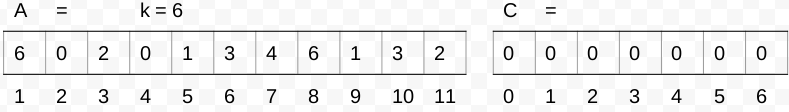
\includegraphics[width=0.8\textwidth]{q5-5-p1}
\end{figure}
\\
O vetor $A$ nunca é alterado, o vetor $C$ é representado abaixo após o final do 
segundo laço (esquerda) e após o final do terceiro laço (direita):
\begin{figure}[h]
  \centering
    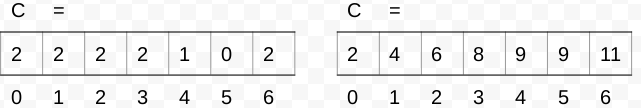
\includegraphics[width=0.8\textwidth]{q5-5-p2}
\end{figure}
\\
O último laço começa pelo com o índice $j = n$ e vai até 1, o vetor B começa 
vázio e vai sendo preenchido até o final do algoritmo. Abaixo segue os estados 
dos vetores $C$ e $B$ no fim das iterações $j = 8, j = 4$ e $j = 1$:
\begin{figure}[h]
  \centering
    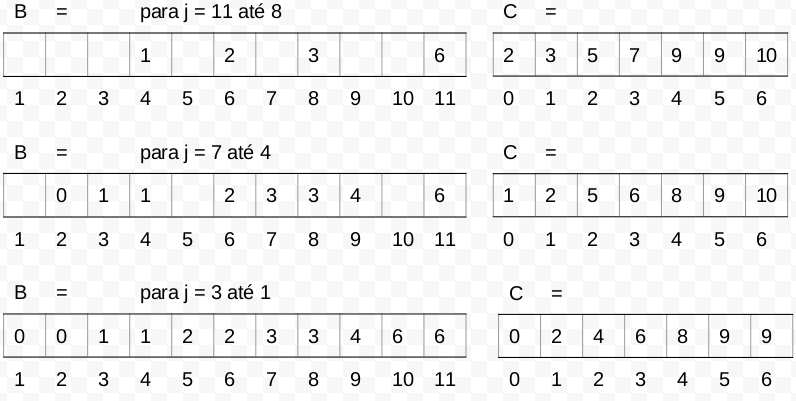
\includegraphics[width=0.8\textwidth]{q5-5-p3}
\end{figure}
\\
Então o algoritmo se encerra mantendo o vetor $B$ ordenado.
\\[12pt]


\noindent 6. (\textbf{CLRS 8.2-2}) Mostre que o \proc{Counting-Sort} é estável.\\[6pt]

Vimos em sala que um algoritmo de ordenação é estável se sempre que, inicialmente, $A[i] = A[j]$ para $i < j$, a cópia $A[i]$ termina em uma posição menor do vetor que a cópia $A[j]$. 

O \proc{Counting-Sort} conta quantas vezes um inteiro de $1..k$ aparece em $A[1..n]$ e armazena essa informação no vetor $C$. A próxima iteração faz com que o vetor $C$ tenha a contagem acumulada dos elementos em A. Logo, após essa iteração nós sabemos que $C[i] < C[i + 1]$.

A última iteração ordena efetivamente $A$, copiando seus elementos de $n..1$ para um vetor auxiliar $B$. Como a contagem foi feita na ordem $1..n$ e os valores de $C$ são usados como índices em $B$ e eles são decrementados a cada vez que uma cópia é feita, a ordem relativa em que os elementos aparecem em $A$ é preservada, mesmo no caso onde há repetições, garantindo, assim, a estabilidade do algoritmo.\\[12pt]


\noindent 8. (\textbf{CLRS 8.2-4}) Descreva um algoritmo que, dados $n$ inteiros 
no intervalo de $1$ a $k$, preprocesse sua entrada e então responda em $O(1)$ 
qualquer consulta sobre quantos dos $n$ inteiros dados caem em um intervalo $[a 
\cdots b]$. O preprocessamento efetuado pelo seu algoritmo deve consomir tempo 
$O(n + k)$.
\\[6pt]
\textbf{Resposta}: O algoritmo desenvolvido é baseado no algoritmo de 
\textit{Counting Sort} descrito no livro do Cormen. O algoritmo possuí duas 
rotinas, uma de preprocessamento que devolve um vetor de contagem C e um de 
consulta que retorna a quantidade de elementos conforme o enunciado. O algoritmo 
de preprocessamento abaixo recebe um vetor $A$ de $n$ inteiros qualquer tal que 
seus elementos estão dentro do intervalo $[1 \cdots k]$ e  realiza o 
preprocessamento devolvendo o vetor "$C$" do \textit{counting sort} antes de 
ordena-lo no vetor $B$. Esse vetor possuí o índice do último valor no vetor 
ordenado de cada índice, por exemplo, $C[x] = y$, indica que o último elemento 
$x$ está no índice $y$ do vetor ordenado.

\begin{codebox}
\Procname{$\proc{PreProcessamento}(A, k, n)$}
\li    \For $i \gets 1$ \To $k$
\li    \Do
            $C[i] \gets 0$
       \End
\li    \For $i \gets 1$ \To $n$
\li    \Do
            $C[A[i]] \gets C[A[i]] + 1$
       \End
\li    \For $i \gets 2$ \To $k$
\li    \Do
            $C[i] \gets C[i] + C[i-1]$
       \End
\li    \Return $C$
\End
\end{codebox}
O procedimento $\proc{ContaNoIntervalo}$ recebe o vetor gerado pelo 
$\proc{PreProcessamento}$ e os extremos do intervalo $[a \cdots b]$ e devolve a 
quantidade de elementos do vetor original $A$ que estão dentro desse vetor.
\begin{codebox}
\Procname{$\proc{ContaNoIntervalo}(C, a, b)$}
    \li \If $a \leq 1$
    \li     \Then
            $a' \gets 1$
    \li \Else
            $a' \gets C[a-1] + 1$
        \End
    \li \Return $C[b] - a' + 1$
\End
\end{codebox}
\textbf{Corretude}
\\[6pt]
O procedimento de preprocessamento utiliza o \textit{counting sort} disso 
sabemos que o vetor $C[i]$ contém a quantidade de elementos menores ou iguais a 
$i$ do vetor original, isso implica que o valor de $C[i]$ é a posição do último 
elemento $i$ (não o elemento da posição $i$) do vetor original no vetor 
ordenado, isso implica também que o valor de $C[i-1] + 1$ é a posição do 
primeiro elemento $i$ do vetor original $A$ no vetor ordenado. Disso temos que 
$C[b] - C[a-1] + 1$ é quantidade de elementos com os valores entre $[a \cdots 
b]$ do vetor original. Note que o $if$ do procedimento 
$\proc{ContaNoIntervalo}$, apenas garante que $a-1 \geq 1$ para que não seja 
acessado uma posição fora do vetor $C$, caso isso ocorra consideramos que a 
posição inicial é $1$, note que isso é válido para quando existem valores $1$ em 
$A$ e quando não existem.
\\[6pt]
\textbf{Desempenho}
\\[6pt]
Veja a tabela de gastos em cada linha do procedimento $\proc{PreProcessamento}$:

\begin{table}[H]
\centering
\begin{tabular}{|l|l|}
\hline
Linha                   & Tempo \\ \hline
1 & $\Theta(k)$ \\ \hline
2 & $\Theta(k)$ \\ \hline
3 & $\Theta(n)$ \\ \hline
4 & $\Theta(n)$ \\ \hline
5 & $\Theta(k)$ \\ \hline
6 & $\Theta(k)$ \\ \hline
7 & $\Theta(1)$ \\ \hline
Total & $\Theta(n + k)$ \\ \hline
\end{tabular}
\end{table}
\noindent O procedimento gasta o tempo total $\Theta(n + k)$. O tempo gasto no 
procedimento $\proc{ContaNoIntervalo}$ está expresso na tabela abaixo:
\begin{table}[H]
\centering
\begin{tabular}{|l|l|}
\hline
Linha                   & Tempo \\ \hline
1 & $\Theta(1)$ \\ \hline
2 & $\Theta(1)$ \\ \hline
3 & $\Theta(1)$ \\ \hline
4 & $\Theta(1)$ \\ \hline
Total & $\Theta(1)$ \\ \hline
\end{tabular}
\end{table}
\noindent Portanto o algoritmo gasta tempo $\Theta(n + k)$ para o 
preprocessamento e tempo $\Theta(1)$ para a chamada a contagem dos elementos 
conforme enunciando do exercício.
\clearpage

\begin{center} 
\textbf{\large{CLRS (Outros)}}
\end{center}


\noindent A.1-7 Avalie o produtório $\prod_{k=1}^n 2(4^k)$.\\[6pt]
\begin{align*}
\prod_{k=1}^n 2(4^k) = \prod_{k=1}^n 2({(2^2)}^k) = \prod_{k=1}^n 2(2^{2k}) = \prod_{k=1}^n 2^{2k + 1}
\end{align*}

Se avaliarmos o produtório para $n = 3$, por exemplo:
\begin{align*}
\prod_{k=1}^n 2^{2k + 1} = 2^{2 + 1} \times 2^{4 + 1} \times 2^{6 + 1}
\end{align*}

Percebemos que o expoente de 2 cresce em uma série aritmética:
\begin{align*}
\sum_{k=1}^n 2k + 1 = \sum_{k=1}^n 2k + \sum_{k=1}^n 1 = 2\sum_{k=1}^n k + n =
2(\frac{n(n + 1)}{2}) + n = n(n + 2)
\end{align*}

Portanto:
\begin{align*}
\prod_{k=1}^n 2(4^k) = 2^{n(n + 2)}
\end{align*}

\end{document}